% -*- TeX:de -*-
\NeedsTeXFormat{LaTeX2e}
\documentclass[12pt,a4paper]{article}
\usepackage[german]{babel} % german text
\usepackage[DIV12]{typearea} % size of printable area
\usepackage[T1]{fontenc} % font encoding
%\usepackage[latin1]{inputenc} % most likely on Windows
\usepackage[utf8]{inputenc} % probably on Linux
\usepackage{multicol}

% PLOTTING
\usepackage{pgfplots} 
\usepackage{pgfplotstable}
\usepackage{url}
\usepackage{graphicx} % to include images
\usepackage{tikz}
\usepackage{subfigure} % for creating subfigures
\usepackage{amsmath} % a bunch of symbols
\usepackage{amssymb} % even more symbols
\usepackage{booktabs} % pretty tables

% a floating environment for circuits
\usepackage{float}
\usepackage{caption}

%\newfloat{circuit}{tbph}{circuits}
%\floatname{circuit}{Schaltplan}

% a floating environment for diagrams
%\newfloat{diagram}{tbph}{diagrams}
%\floatname{diagram}{Diagramm}

\selectlanguage{german} % use german

\begin{document}

%%%%%%% DECKBLATT %%%%%%%
\thispagestyle{empty}
			\begin{center}
			\Large{Fakultät für Physik}\\
			\end{center}
\begin{verbatim}


\end{verbatim}
							%Eintrag des Wintersemesters
			\begin{center}
			\textbf{\LARGE WS 2013/14}
			\end{center}
\begin{verbatim}


\end{verbatim}
			\begin{center}
			\textbf{\LARGE{Physikalisches Praktikum\\ für das Bachelorstudium}}
			\end{center}
\begin{verbatim}




\end{verbatim}

			\begin{center}
			\textbf{\LARGE{PROTOKOLL}}
			\end{center}
			
\begin{verbatim}





\end{verbatim}

			\begin{flushleft}
			\textbf{\Large{Experiment (Nr., Titel):}}\\
							%Experiment Nr. und Titel statt den Punkten eintragen
			\LARGE{PW4 Oberflächenspannung, Viskosität, Hygrometrie, Schmelzwärme}	
			\end{flushleft}

\begin{verbatim}

\end{verbatim}	
							%Eintragen des Abgabedatums, oder des Erstelldatums des Protokolls
			\begin{flushleft}
			\textbf{\Large{Datum:}} \Large{31.10.2013}
			\end{flushleft}
			
\begin{verbatim}
\end{verbatim}
							%Namen der Protokollschreiber
		\begin{flushleft}
			\textbf{\Large{Namen:}} \Large{Patrick Braun, Johannes Kurz}
			\end{flushleft}

\begin{verbatim}


\end{verbatim}
							%Kurstag und Gruppennummer, zb. Fr/5
			\begin{flushleft}
			\textbf{\Large{Kurstag/Gruppe:}} \Large{DO/2}
			\end{flushleft}

\begin{verbatim}



\end{verbatim}
							%Name des Betreuers, das Praktikum betreute.
			\begin{flushleft}
			\LARGE{\textbf{Betreuer:}}	\Large{ Franz Sachslehner }	
			\end{flushleft}

%%%%%%% DECKBLATT ENDE %%%%%%%
\pagebreak
\setlength{\columnsep}{20pt}
\begin{multicols}{2}
\section{Einleitung}

\section{Oberflächenspannung}
Ziel des Experiments ist es die Oberflächenspannung einer Flüssigkeit zu bestimmen. Dazu wird ein Metallring an einer Waage befestigt und mit einer Skala und Gewichten geeicht. Taucht man den Ring in die Flüssigkeit und zieht den Flüssigkeitsbehälter langsam nach unten, kann beim Reißen der sich bildenden Flüssigkeitsmembran an der Skala die Kraft abgelesen werden. Den Aufbau und die Eichgewichte sind in Abbildung \ref{fig:oberflaeche_eichung_aufbau} ersichtlich.
\begin{figure}[H]
	\centering
	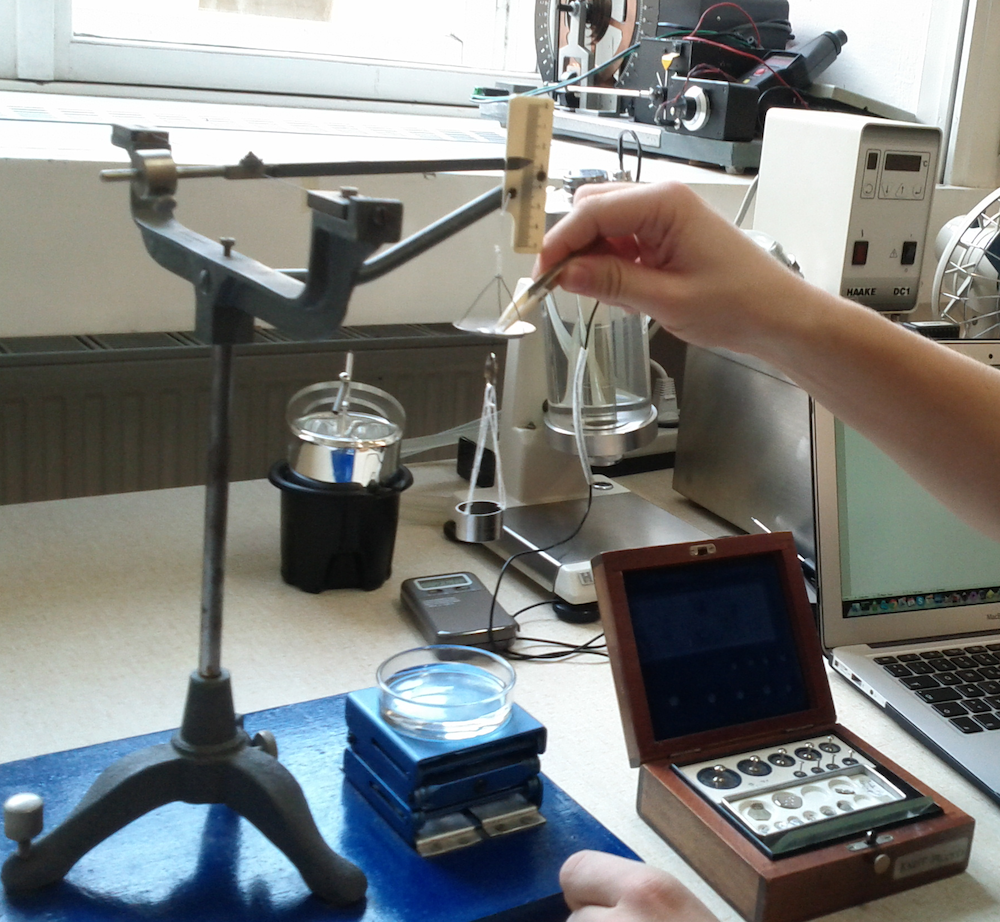
\includegraphics[scale=0.2]{./figure/Waageneichung-Aufbau.png}
	\caption{Foto \\Versuchsaufbau und Eichung}
	\label{fig:oberflaeche_eichung_aufbau}
\end{figure}
\noindent
Bevor Messungen durchgeführt werden können muss wie erwähnt die verwendete Waage geeicht werden. Dazu werden auf die Schale welche zwischen Ring und Befestigung angebracht ist, 0.1g schwere Metallstücke gelegt und die dazugehörigen Striche abgelesen. Dies wird von 0.1g bis 1.4g durchgeführt. Dadurch kann die Kraft pro Strich mit
$$K = m * a$$
errechnet werden. K ist ein empirischer wert den wir bei der Messung von der Skala ablesen.
Weiters ist die Oberflächenspannung abhängig von der Fläche des Ringes. Das Verhältnis zwischen Zugkraft und Fläche ergibt die Oberflächenspannung:
$$\sigma = \frac{K}{\pi * (d_1 + d_2)}$$
\noindent
Folgende Materialien wurden verwendet:
\begin{itemize}
	\item Eichgewichter
	\item Eine Pinzette
	\item Eine Waage
	\item Schale mit Wasser
	\item Metallring mit Aufhängung
	\item Ein beweglicher Objekttisch
\end{itemize}
Bei der Durchführung wurde zu erst normals- und um danach destilliertes Wasser verwendet um einen Vergleich zu ermöglichen. Näheres dazu wird im Punkt Diskussion erläutert.
\subsection{Messwerte und Ergebnisse}
Die Eichung der Waage ergab einen linearen Anstieg (Abbildung \ref{fig:oberflaeche_eichung_fit}) über den wir die Kraft pro Strich im Mittel genau errechnen können.
\begin{figure}[H]
	\centering
	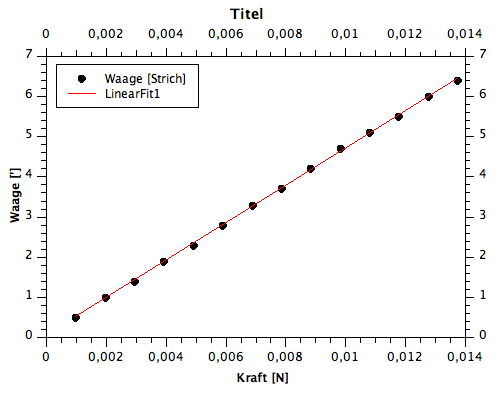
\includegraphics[scale=0.45]{./figure/Waageneichung-Fit.png}
	\caption{Skizze Versuchsaufbau}
	\label{fig:oberflaeche_eichung_fit}
\end{figure}
\noindent
Durch die lineare Regression (Abbildung \ref{fig:oberflaeche_eichung_linreg}) der Messwerte (Tabelle \ref{fig:oberflaeche_eichung}) erhält man die Steigung der Kraft pro strich. Diese Steigung entspricht pro Strich \textbf{$K = \frac{1}{465} = (0.0022\pm 0.000012)N$}. Für den Metallring wurde mit einer Schiebelehre wie folgt gemessen:\\
Außendurchmesser: $(24.00 \pm 0.05)mm$\\
Innendurchmesser: $(23.15 \pm 0.05)mm$\\
Errechnet man sich die Oberflächenspannung zusammen mit den Werten aus Tabelle \ref{fig:oberflaeche_messung} für $Wasser_{destilliert}$ ergibt sich:
$$\sigma = \frac{4.62 * 0.0022N}{\pi * (0.02400 + 0.02315)m} =$$ 
$$= (68.62 \pm 0.36) \frac{mN}{m}$$ %TODO Fehler
Für Wasser mit Verunreinigungen: 
$$ \sigma = \frac{3.9 * 0.0022N}{\pi * (0.02400 + 0.02315)m} =$$
$$ = (57.92 \pm 0.33) \frac{mN}{m}$$



% Regress in Strich gegen N
%%%B (y-intercept) = -1,343535761669278e-04 +/- 4,628591085282343e-05
%%%A (slope) = 2,149302255457725e-03 +/- 1,174365191704868e-05


\begin{figure}[H]
	\centering
	\pgfplotstabletypeset[
			columns={g,strich},
			col sep=tab,
			columns/T1/.style={column name=$T_1[s]$},
			columns/T2/.style={column name=$T_2[s]$},
			every head row/.style={before row=\hline,after row=\hline\hline},
			every last row/.style={after row=\hline},
			every first column/.style={
								column type/.add={|}{}
							        },
			every last column/.style={
								column type/.add={}{|}
								}
			]{./data/oberflaechenspannung_eichung.dat}
	\caption{Eichungsmessung der Waage}
	\label{fig:oberflaeche_eichung}
\end{figure}
\noindent

\begin{figure}[H]
	\centering
	\pgfplotstabletypeset[
			col sep=space,
			every head row/.style={before row=\hline,after row=\hline\hline},
			every last row/.style={after row=\hline},
			every first column/.style={
								column type/.add={|}{}
							        },
			every last column/.style={
								column type/.add={}{|}
								}
			]{
			Wasser $Wasser_{destilliert}$
			3.9 4.7
			3.8 4.6
			3.9 4.6
			3.9 4.6
			3.9 4.6
			3.9 0
			4.0 0
			}
	\caption{Messung von Wasser und destilliertem Wasser}
	\label{fig:oberflaeche_messung}
\end{figure}
\noindent
\\
Temperatur erste Messung:\\
$23.5^{\circ}C$\\
Temperatur zweite Messung:\\
$22.3^{\circ}C$\\
\subsection{Diskussion}
Die Durchführung der Eichung und Messung gestaltete sich unproblematisch. Die Eichung erfordert etwas Fingerspitzengefühl und Geduld da die Waage einen (fast) umgedämpften Oszillator gleicht. Bei den ersten Zwischenrechnungen ergab sich ein zu niedriger Wert im Vergleich zum Literaturwert. \\
Literaturwert: \\
Wasser bei $20^{\circ}$ $\sigma = 72.75 \frac{mN}{m}$.\\
Daraufhin wurde das Wasser in der Schale nach der Reinigung derselben durch destilliertes Wasser ersetzt um die Verunreinigungen so niedrig wie möglich zu halten. Zusätzlich war das Wasser um ca. $1^{\circ}C$ kühler was ebenfalls zu einer Näherung an den Literaturwert geführt hat. Mit einem Wert von $(69 \pm 0.2) \frac{mN}{m}$ liegt die Messung bei $22.3^{\circ}C$ bei einem zu erwartenden Wert. Die Differenz ist hauptsächlich durch den Temperaturunterschied zu erklären und an den Messungenauigkeiten der verwendeten Geräte. %TODO Fehler

%%%%%%%%%%%%%%%%%%%%%%%%%%%%%%%%%%%%
\section{Viskosität}


%%% TO DO Handskizze Stokesversuch


Rühre, Pinzette, Kugeln
Thermometer Sumit DT150\\
\subsection{Messwerte und Ergebnisse}
Temp: $24^{\circ}C \pm 1^{\circ}C$\\
Länge Innen-Innen: 13.42cm\\
Dichte Flüssigkeit: $1225 \pm 5 kg/m^2$\\
\\
Messungen 1:\\
$0.794 \pm 0.002mm$\\
$16.1 \pm 0.1 mg$\\
Messung 2:\\
$6.6 \pm 0.1mg$\\
$0.595 \pm 0.01mm$\\
Fallzeiten:\\
\begin{figure}[H]
	\centering
	\pgfplotstabletypeset[
			col sep=space,
			every head row/.style={before row=\hline,after row=\hline\hline},
			every last row/.style={after row=\hline},
			every first column/.style={
								precision=2,
								column type/.add={|}{}
							        },
			every last column/.style={
								precision=2,
								column type/.add={}{|}
								}
			]{
			$Messung_1 Messung_2$
			2.40 3.94
			2.37 3.97
			2.40 3.97
			2.38 4.13
			2.41 3.97
			2.41 3.97
			2.31 3.97
			2.44 3.79
			2.47 3.97
			2.44 3.88
			2.47 4.04
	}
	\caption{Messung von Fallzeiten}
	\label{fig:visko_fallzeit}
\end{figure}
\noindent
\textbf{Höppler-Viskosimeter}\\
HAAKE, Thermometer, Heizgerät\\
Temperatur: $25.0^{\circ}C \pm 0.1^{\circ}C$\\
Messung 1: 2m51s90ms\\
Messung 2: 2m51s32ms\\
Messung 3: 2m51s32ms\\
\\
Temperatur: $50.6^{\circ}C \pm 0.1^{\circ}C$\\
Messung 1: 0m42s25ms\\
Messung 2: 0m41s63ms\\
Messung 3: 0m41s78ms\\
\\
\subsection{Diskussion}


%%%%%%%%%%%%%%%%%%%%%%%%%%%%%%%%%%%%
\section{Luftfeuchtigkeit}
\subsection{Messwerte und Ergebnisse}
$T_{Start} = 24^{\circ}C \pm 1^{\circ}C$\\

\subsection{Diskussion}


%%%%%% EIS - SCHMELZWAERME %%%%%%%%

\section{Schmelzwärme vonEis}
Bei der Wärmezufuhr in einen Stoff kommt es bei Phasenübergängen zu Zeiten konstanter Temperatur, währendderer die zugeführte Energie zur Gänze in die Zustandsänderung, nicht jedoch in die Temperaturänderung geht.\\
\\
In diesem Versuch soll die spezifische Schmelzwärme von Eis (Wasser aus der Haushaltsleitung, Wien) bestimmt werden. Es wird dazu die Mischungsmethode verwendet:\\
In einem (idealerweise völlig) wärmeisolierten Gefäß werden 2 Stoffe unterschiedlicher Temperatur gemischt. Die abgegebene Wärmemenge des wärmeren Stoffes muss wegen der Energieerhaltung gleich der aufgenommenen Wärmemenge des kälteren und des Gefäßes sein.\\
Aus den Anfangstemperaturen und der Mischtemperatur lässt sich beispielsweise auf die latente Wärme schließen, die beim Schmelzvorgang von Eis frei wird.
$$\Delta Q_1=(C_k+m_wc_w)(T_1-T_m)=$$
$$=\Delta Q_2 = m_eS+m_ec_w(T_m-T_S)$$
$S$ ist die gesuchte spezifische Schmelzwärme des Eises, die Massen $m_e$, $m_w$ des verwendeten Wasser und Eises sowie die Wärmekapazitäten $c_w$, $C_k$ von Wasser und dem verwendeten Gefäß gehen in die Rechnung ein.\\

%%%% TO DO Handskizze Kalorimeter

\noindent Equipment:
\begin {itemize}
	\item Ein Kalorimetergefäß mit Rührer
	\item Wasser und Eis
	\item Ein ULab-Datalogger mit Temperatursonde
\end {itemize}

Das Kalorimeter wird, zu etwas mehr als der Hälfte, mit erhitztem Wasser (ca. $80^{\circ}$ C) gefüllt und der Temperaturverlauf des Systems wird mehrere Minuten gemessen.\\
Nach ein paar Minuten wird Eis eingebracht (weniger als Wasser). Es ist darauf zu achten, das Eis schnell einzuwerfen und sofort und durchgehend zu rühren um den Schmelzvorgang zu beschleunigen.\\
Schließlich soll ein instantaner Temperaturausgleich approximiert werden.\\
Während des gesamten Versuchs wird der Temperaturverlauf gemessen, der grob in 3 Abschnitte geteilt werden kann, die durch Anlegen von Geraden idealisiert werden (vgl. Abb. \ref{fig:Tempverlauf-Eis}):\\
- Vor der Zugabe von Eis\\
- während des Schmelzvorganges\\
- nach der Vermischung


\end{multicols}

%%%% Diagramm Eis
\begin{figure}[H]
	\centering
	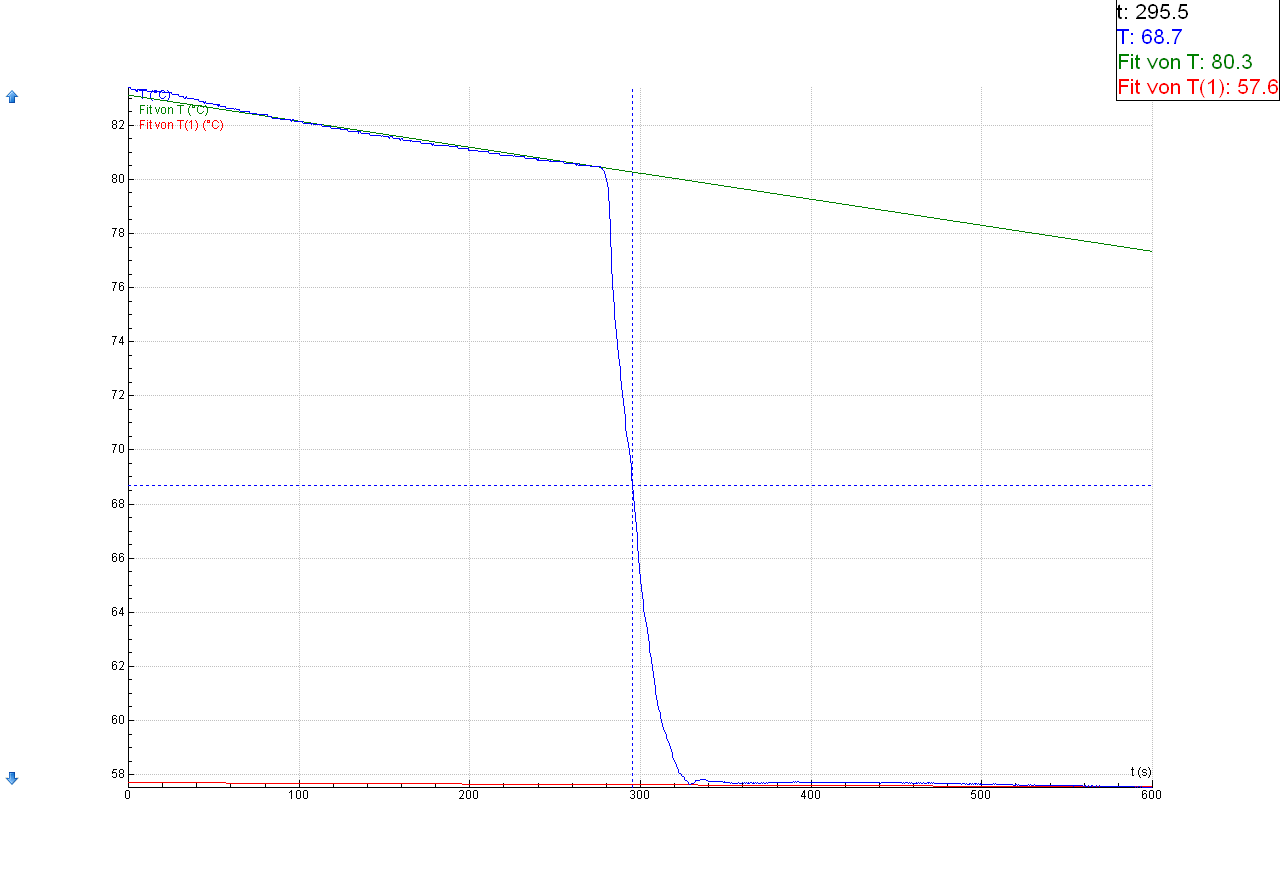
\includegraphics[scale=0.35]{./figure/PW4_graph.PNG}
	\caption{Temperatur in [$^\circ$C] gegen die Zeit in [s] im Kalorimeter\ }
	{\centering Screenshot aus Coach6}
	\label{fig:Tempverlauf-Eis}
\end{figure}
\noindent

\begin{multicols}{2}


\subsection{Messwerte und Ergebnisse}

\begin{itemize}
	\item Wärmekapazitäten:\\
	Kalorimeter: $C_k = (100 \pm 10) J/K$\\
	Wasser (20$^{\circ}$C): $c_w=(4,182) J/gK$
	
	\item Massen:\\
	Kalorimeter: $(236.6 \pm 0.1)g$\\
	Wasser: $m_w = (154.0 \pm 0.2)g$\\
	Eis: $m_e = (26.0 \pm 0.2)g$
	
	\item Temperaturen:\\
	Anfang: $T_1=(80 \pm 1) ^\circ C$\\
	Ende: $T_m=(58 \pm 1) ^\circ C$\\
	Schmelztemp. Eis: $T_S = 0 ^\circ C$
\end{itemize}

\noindent spezifische Schmelzwärme von Wasser:\\
$$S =(387 \pm 45) kJ/kg$$

\subsection{Diskussion}
Der Literaturwert der spezifischen Schmelzwärme von Eis von 333.5 KJ/kg liegt außerhalb des Unsicherheitsbereichs dieser Messung:\\
Die angewandte Methode bietet, trotz computergestützter Messung, einige mögliche Fehlerursachen:\\
Die horizontalen Geraden in Abb \ref{fig:Tempverlauf-Eis} wurden "von Hand" gefittet und die Flächen links und rechts der senkrechten Schnittgerade als gleich abgeschätzt. Hier sind sicherlich Verbesserungen möglich, auch wenn die Fehlerabschätzung von $\pm 1 ^\circ C$ bei beiden Temperaturen bewusst groß gewählt ist, um dem Problem gerecht zu werden.\\
\\
Eine andere Fehlerquelle hat sich sehr deutlich in einem ersten Versuch gezeigt, in dem sowohl das Einbringen der Eiswürfel sehr zögerlich und langsam durchgeführt wurde, als auch vergessen wurde, zu rühren, um die Vermischung zu beschleunigen. Dadurch ergaben sich unerwartete und große Temperaturschwankungen im Schmelzzeitraum und das Experiment musste wiederholt werden.\\
Es ist also durchaus möglich, dass das Öffnen der Abdeckung zum Eiswürfel-Input, und andere Manipulationen am System (rühren, messen, Wärmeleitung des Kalorimeters, u.a.) auch zu Verzerrungen der Messung führen.\\
Eine weiterer, in dieser Durchführung nicht kontrollierter Parameter in diesem Experiment ist das verwendete Wasser: Es wurde Wasser aus der Wiener Haushaltswasserleitung verwendet, ohne etwaige Bestandteile genauer zu ermitteln. Das Wasser wurde erhitzt im Wasserkocher der Praktikumsräume, auch hier sind Verunreinigungen nicht auszuschließen.\\
Um also den Einfluss einzelner der erwähnten Fehlerquellen zu bestimmen und diese zu minimieren, wären also weitere Versuche, unter verschiedenen Bedingungen, nötig. Beispielsweise könnte das Experiment mit destilliertem Wasser durchgeführt werden, die gemessenen Daten mit unterschiedlichen Programmen ausgewertet und die Durchführung durch Übung und Verwendung eines anderen Gefäßes beschleunigt werden.


\section{Quellen}
Formeln und Abbildung Fahrradpendel:\\
\url{http://www.univie.ac.at/anfpra/neu1/pw/pw3/PW3.pdf}\\

\noindent spezifische Wärmekapazität von Wasser:\\
\url{http://de.wikipedia.org/wiki/Spezifische_W%C3%A4rmekapazit%C3%A4t}

\end{multicols}
\end{document}